%*****************************************
\chapter{Formulas}\label{ch03:formulas}
%*****************************************

Excel workbooks are designed to create useful and complex calculations. In addition to doing arithmetic, Excel can look up data and display results based on logical conditions. Finally, Excel can highlight specific results to enhance analysis. These skills will be demonstrated in the context of a typical grade book spreadsheet that contains the results for an imaginary Excel class.

\begin{center}
	\begin{objbox}{Learning Objectives}
		\begin{itemize}
			\setlength{\itemsep}{0pt}
			\setlength{\parskip}{0pt}
			\setlength{\parsep}{0pt}

			\item Use the \textit{Quick Analysis Tool} to find the Total Points and Points Possible for all students.
			\item Write a division formula to find the Percentage for each student, using an absolute reference to the \textit{Total Points Possible}.
			\item Write an \textit{IF} Function to determine Pass/Fail where passing is $ 70\% $ or higher.
			\item Write a \textit{VLOOKUP} to determine the Letter Grade using a Letter Grades scale.
			\item Use the \textit{TODAY} function to insert the current date.
			\item Review common Error Messages using \textit{Smart Lookup} to get definitions of some of the terms in the spreadsheet.
			\item Apply \textit{Data Bars} to the Total Points values.
			\item Apply \textit{Conditional Formatting} to the Percentage, Pass/Fail, and Letter Grade columns.
			\item Printing Review – Change to Landscape, Scale to Fit Columns on One Page and Set Print Area.
			
		\end{itemize}
	\end{objbox}
\end{center}

Figure \ref{03:fig01} shows the completed workbook that will be demonstrated in this chapter. Notice the techniques used in \textit{Column O} and \textit{Column R} that highlight the results of the calculations. Notice, also that there are more numbers on this version of the file than in the original data file. These are all completed using Excel calculations.

\begin{figure}[H]
	\centering
	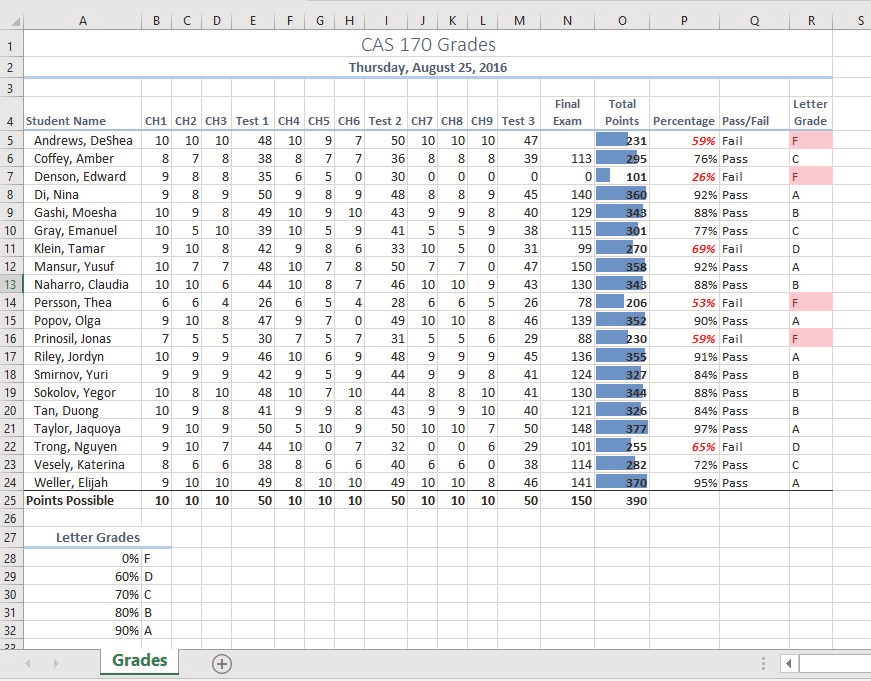
\includegraphics[width=\maxwidth{.95\linewidth}]{gfx/ch03_fig01}
	\caption{Completed Grade Book Worksheet}
	\label{03:fig01}
\end{figure}

\section{More on Formulas and Functions}

\begin{center}
	\begin{objbox}{Learning Objectives}
		\begin{itemize}
			\setlength{\itemsep}{0pt}
			\setlength{\parskip}{0pt}
			\setlength{\parsep}{0pt}
			
			\item Review the use of the \textit{=MAX} function.
			\item Examine the \textit{Quick Analysis Tool} to create standard calculations, formatting, and charts very quickly.
			\item Create Percentage calculation.

			\begin{itemize}
				\setlength{\itemsep}{0pt}
				\setlength{\parskip}{0pt}
				\setlength{\parsep}{0pt}

				\item Use the \textit{Smart Lookup} tool to acquire additional information about percentage calculations.
				\item Review the use of Absolute cell reference in a division formula.
			\end{itemize}

		\end{itemize}
	\end{objbox}
\end{center}

\subsection{Another Use for \fmtTyping{=MAX}}

Before moving on to the more interesting calculations discussed in this chapter, it is necessary to determine how many points it is possible for each student to earn for each of the assignments. This information will go into \textit{Row} $ 25 $. The \textit{=MAX} function is the tool of choice for this task.

\begin{enumbox}
	\begin{enumerate}
		\item Open the data file \fmtWorksheet{CH3-Data} and save the file as \fmtWorksheet{CH3-Grade Book}.
		\item Click \fmtLoc{B25}.
		\item Start typing \fmtTyping{=MAX} (See Figure \ref{03:fig02}). Note the explanation that pops up on the offered list of functions. Either keep typing \fmtTyping{(} (an open parenthesis) or double click \fmtButton{MAX} from the popup list.

		\begin{figure}[H]
			\centering
			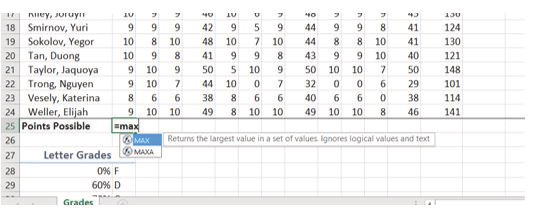
\includegraphics[width=\maxwidth{.95\linewidth}]{gfx/ch03_fig02}
			\caption{Entering a function}
			\label{03:fig02}
		\end{figure}
	
		\item Select the range \fmtLoc{B5:B24}. The calculation will update to: \fmtTyping{=MAX(B5:B24)}. Press \fmtKeystroke{Enter} to complete the formula.
		\item Now, use the \fmtButton{Auto Fill Handle} to copy \fmtLoc{B25} to \fmtLoc{C25:N25}. Note that as the calculation is copied from one column to the next, the cell references change. The calculation in \fmtLoc{B25} reads: \fmtTyping{=MAX(B5:B24)} and the one in \fmtLoc{N25} reads \fmtTyping{=MAX(N5:N24)}. These cell references are called \textit{relative} references.
	\end{enumerate}
\end{enumbox}

By default, the calculations that Excel copies change their cell references relative to the row or column they are copied to. That makes sense. \textit{Column N} should not display an answer that uses the values from \textit{Column K}.

To see all the calculations that were just created, press \fmtKeystroke{Ctrl} + \fmtKeystroke{$ ` $} (that is the back-tic near the \fmtKeystroke{one} on the keyboard, see Figure \ref{03:fig03}) \fmtKeystroke{Ctrl} + \fmtKeystroke{$ ` $} displays the calculations (formulas) in each cell. Pressing \fmtKeystroke{Ctrl} + \fmtKeystroke{$ ` $} a second time will display calculations as values, which is the default view for cells.

\begin{figure}[H]
	\centering
	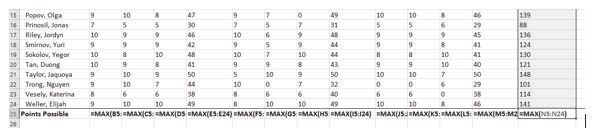
\includegraphics[width=\maxwidth{.95\linewidth}]{gfx/ch03_fig03}
	\caption{Relative References – Displayed as calculations.}
	\label{03:fig03}
\end{figure}

\subsection{Quick Analysis Tool}

The \textit{Quick Analysis Tool} creates standard calculations, formatting, and charts very quickly. In this exercise, it is used to insert the \textit{Total Points} for each student in \textit{Column O}.

If necessary, press \fmtKeystroke{Ctrl} + \fmtKeystroke{$ ` $} to return the spreadsheet to the normal view (the results of the formulas in \textit{Row }$ 25 $ should be displayed, not the formulas themselves).

\begin{enumbox}
	\begin{enumerate}
		\item Select \fmtLoc{B5:N25}
		\item In the lower right corner of the selection, notice the \fmtButton{Quick Analysis Tool} (see Figure \ref{03:fig04}).
	
		\begin{figure}[H]
			\centering
			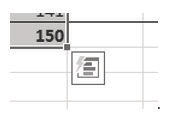
\includegraphics[width=\maxwidth{.95\linewidth}]{gfx/ch03_fig04}
			\caption{Quick Analysis Tool}
			\label{03:fig04}
		\end{figure}
	
		\item In the \fmtButton{Quick Analysis Tool}, select \fmtButton{Totals $ \Rightarrow $ COLUMN SUM} (see Figure \ref{03:fig05}). (Note: there are two SUM buttons, the second will sum columns, as indicated by the tan-colored column indicator on the button.) Selecting the \fmtButton{COLUMN SUM} button places a \fmtTyping{=SUM()} calculation all cells in \fmtLoc{Column O}.
	\end{enumerate}
\end{enumbox}

\begin{figure}[H]
	\centering
	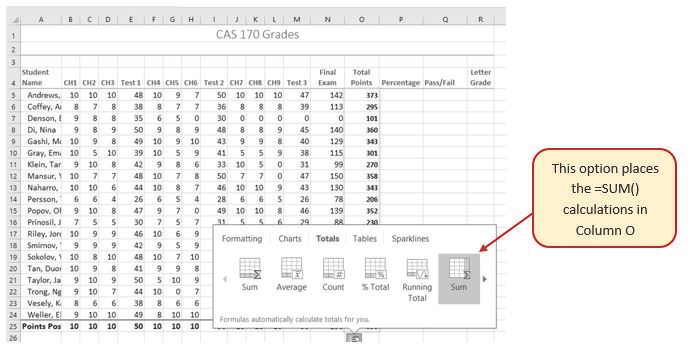
\includegraphics[width=\maxwidth{.95\linewidth}]{gfx/ch03_fig05}
	\caption{Quick Analysis Tool – Totals, Sum Column}
	\label{03:fig05}
\end{figure}

\subsection{Percentage Calculation}

\textit{Column P} requires a Percentage calculation. Before creating a calculation for this, it might be handy to know precisely what is needed. The \textit{Smart Lookup} tool is a handy way to get more information if the computer is connected to the Internet.

\begin{enumbox}
	\begin{enumerate}
		\item Select cell \fmtLoc{P4}.
		\item Click \fmtButton{Review $ \Rightarrow $ Insights $ \Rightarrow $ Smart Lookup} (see Figure \ref{03:fig06}). This will find more about Percentage calculations. If this is the first time that the \textit{Smart Lookup} tool has been used a privacy statement may pop up. Press the \fmtButton{Got it} button.
	\end{enumerate}
\end{enumbox}
	
Excel searches the web for articles relevant to \textit{percentage} and lists links to those articles. Figure \ref{03:fig06} illustrates the result of the search done when this lesson was written, but that result will change depending on what information is available on the web.

\begin{figure}[H]
	\centering
	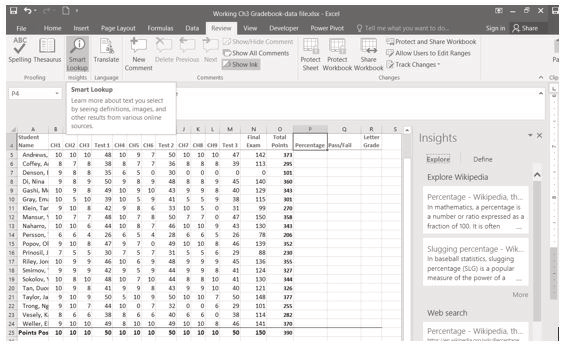
\includegraphics[width=\maxwidth{.95\linewidth}]{gfx/ch03_fig06}
	\caption{Smart Lookup tool}
	\label{03:fig06}
\end{figure}

Now that the data needed for the \textit{Percentage} calculation is known, a formula can be written so Excel will complete the calculation. The \textit{Total Points} for each student must be divided by the \textit{Total Points Possible}. Notice that there is a different number of points earned for each student, but there is only one \textit{Total Points Possible} --- the value in cell $ O25 $.

\begin{enumbox}
	\begin{enumerate}
		\item Click in \fmtLoc{P5}.
		\item Press \fmtTyping{=} then click \fmtLoc{O5}. 
		\item Enter \fmtTyping{/}
		\item Click \fmtLoc{O25}. The calculation should look like \fmtTyping{=O5/O25}.
		\item Press \fmtKeystroke{Enter}. The result of the formula should be $ 0.95641026 $. So far, so good. DeShea Andrews is doing well in this class, with a percentage grade of almost 96\%---definitely an ``A''!)
		\item Next use the \fmtButton{Auto Fill Handle} to copy the calculation from \fmtLoc{P5} to \fmtLoc{P6:P24} to calculate the other students' grades. Unfortunately, this error message is displayed: \textit{\#DIV/$ 0 $}. This message means that an attempt has been made to divide a number by $ 0 $ (zero), which is impossible. The formula in \fmtLoc{P9} reads $ =O9/O29 $. The first cell reference is correct --- it points to Moesha Gashi's total points for the class. But the second reference is wrong. It points to an empty cell, \fmtLoc{O29}.
	\end{enumerate}
\end{enumbox}

\begin{figure}[H]
	\centering
	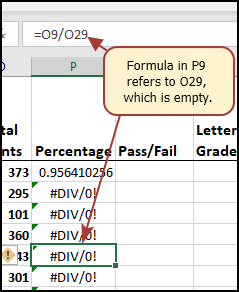
\includegraphics[width=\maxwidth{.50\linewidth}]{gfx/ch03_fig07a}
	\caption{Illegal Cell Reference}
	\label{03:fig07a}
\end{figure}

Before copying the calculation, the second reference, ($ O25 $), must be changed to an absolute cell reference. That way, when it is copied down the column, the cell reference for $ O25 $ will be locked and will not change.

\begin{enumbox}
	\begin{enumerate}
		\item Click in \fmtLoc{P5}. 
		\item In the \textit{Formula Bar} click on \fmtLoc{O25} (see Figure \ref{03:fig07}).
		\item Press \fmtKeystroke{F4} to make the \fmtLoc{O25} reference absolute. That way, it will not change when the cell is copied (see Figure \ref{03:fig08}). It is also easy enough to simply type a \$ before the \fmtLoc{O} and another one before the \fmtLoc{25} for devices like tablets and laptops that may not have function keys.
		\item Press \fmtKeystroke{Enter}.
		\item The formula in \fmtLoc{P5} now looks like \fmtTyping{=O5/\$O\$25}.
		\item Click in \fmtLoc{P5} and use the \fmtButton{Auto Fill Handle} to copy that cell to \fmtLoc{P6:P24}. Now the formula has the correct values for all students.
	\end{enumerate}
\end{enumbox}
	
\begin{figure}[H]
	\centering
	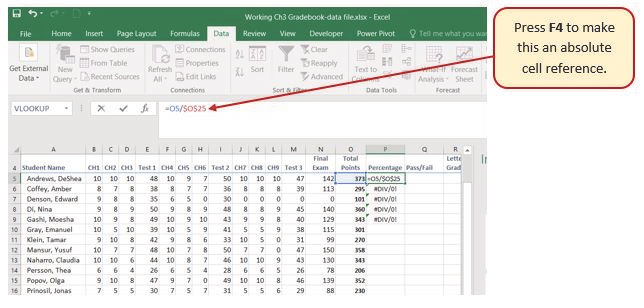
\includegraphics[width=\maxwidth{.40\linewidth}]{gfx/ch03_fig07}
	\caption{Editing a Formula}
	\label{03:fig07}
\end{figure}

\begin{figure}[H]
	\centering
	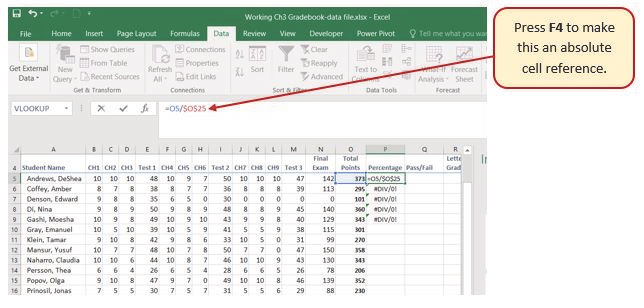
\includegraphics[width=\maxwidth{.40\linewidth}]{gfx/ch03_fig08}
	\caption{Absolute Cell reference – press F4}
	\label{03:fig08}
\end{figure}

Those long decimals in the percent column are nonstandard so they should be changed to a percent by applying cell formatting.

\begin{enumbox}
	\begin{enumerate}
		\item Select the range \fmtLoc{P5:P24}.
		\item Click \fmtButton{Home $ \Rightarrow $ Number $ \Rightarrow $ \% (Percent)}.
	\end{enumerate}
\end{enumbox}

\begin{center}
	\begin{sklbox}{Skill Refresher}
		\textbf{Absolute References}
		\\
		\begin{itemize}
			\setlength{\itemsep}{0pt}
			\setlength{\parskip}{0pt}
			\setlength{\parsep}{0pt}

			\item Click in front of the column letter of a cell reference in a formula or function that should not be altered when the formula or function is pasted into a new cell location.
			\item Press the \fmtKeystroke{F4} key or type a dollar sign (\$) in front of the column letter and row number of the cell reference.
						
		\end{itemize}
	\end{sklbox}
\end{center}

\begin{center}
	\begin{tkwbox}{Key Take-Aways}
		\textbf{Functions}
		\\
		\begin{itemize}
			\setlength{\itemsep}{0pt}
			\setlength{\parskip}{0pt}
			\setlength{\parsep}{0pt}

			\item Functions can be created using cell ranges or selected cell locations separated by commas. Make sure to use a cell range (two cell locations separated by a colon) when applying a statistical function to a contiguous range of cells.
			\item To prevent Excel from changing the cell references in a formula or function when they are pasted to a new cell location, use an absolute reference. Do this by placing a dollar sign (\$) in front of the column letter and row number of a cell reference or by using the \fmtKeystroke{F4} function key.
			\item The \textit{\#DIV/$ 0 $} error appears if a formula attempts to divide a constant or the value in a cell reference by zero, typically because it refers to an empty cell.
			
		\end{itemize}
	\end{tkwbox}
\end{center}

\section{Logical and Lookup Functions}

\begin{center}
	\begin{objbox}{Learning Objectives}
		\begin{itemize}
			\setlength{\itemsep}{0pt}
			\setlength{\parskip}{0pt}
			\setlength{\parsep}{0pt}

			\item Use an \textit{IF} Function to make logical comparisons between a value and what is expected.
			\item Create a \textit{VLOOKUP} calculation to look up information in a table.
			\item Understand error messages.
			\item Understand how to enter and format Date/Time Functions.
			
		\end{itemize}
	\end{objbox}
\end{center}

In addition to doing arithmetic, Excel can do other kinds of functions based on the data in the spreadsheet. In this section an \textit{=IF} function will be used to determine whether a student is passing or failing the class. Then, a \textit{=VLOOKUP} function will be used to determine what grade each student has earned.

\subsection{If Function}

The \textit{IF} function is one of the most popular functions in Excel. It makes logical comparisons between a value and what was expected and then fills a cell based on that comparison. In its simplest form, the \textit{IF} function says something like, \textit{If the value in a cell is expected (true) then do this; otherwise do that}.

The \textit{IF} function has three arguments.

\begin{itemize}
	\item \textbf{Logical test}. This is the test to see if the value in a selected cell expected. A test can be something like ``$ B7=14 $'' or ``$ B7>12 $'' or ``$ B7<6 $.''
	\item \textbf{Value\_if\_true}. What to do if the requirements in the logical test are met, for example, if $ B7 $ is equal to $ 14 $ then fill the cell with text like ``True,'' or ``On budget!'' Alternatively, this argument can contain a calculation, like $ B7*2 $. That is, if $ B7 $ equals $ 14 $ then multiply it by $ 2 $. Finally, if Excel should put nothing at all in the cell then type ``'' (two empty quotes).
	\item \textbf{Value\_if\_false}. What to do if the requirements in the logical test are \textit{NOT} met; for example, if \textit{B7} does \textit{NOT} equal $ 14 $. To have Excel do nothing, then type empty double quotes. Of course, Excel can also enter whatever text or calculation is desired.
\end{itemize}

For the grade book, \textit{Column Q} should indicate whether a student is passing or failing the class. Students who score $ 70\% $ or better are considered passing while scores less than $ 70\% $ are failing.

\begin{enumbox}
	\begin{enumerate}
		\item Click in \fmtLoc{Q5}.
		\item Click \fmtButton{Formulas $ \Rightarrow $ Function Library $ \Rightarrow $ Logical $ \Rightarrow $ IF} (see Figure \ref{03:fig09}).
	\end{enumerate}
\end{enumbox}
	
\begin{figure}[H]
	\centering
	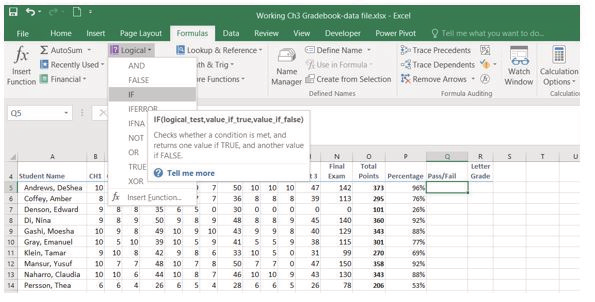
\includegraphics[width=\maxwidth{.95\linewidth}]{gfx/ch03_fig09}
	\caption{IF Function}
	\label{03:fig09}
\end{figure}

The \textit{IF Function} dialog box pops up with a place to enter each of the three arguments.

\begin{enumbox}
	\begin{enumerate}
		\item Click in the box for \fmtButton{Logical Test}. To test whether a student's score is less than $ 0.7 $ enter \fmtTyping{$ P5<0.7 $}.
		\item Click in the box for \fmtButton{Value\_if\_true}. If the student's score is less than $ 0.7 $, then they are failing the class. In this box, type \fmtTyping{Fail}. Note: Excel automatically encloses the word \textit{Fail} in quote marks.
		\item Click in the box for \fmtButton{Value\_if\_false}. If the student's score is \textit{NOT} less than $ 0.7 $, then they are passing the class. In this box, type \fmtTyping{Pass}. Note: Excel automatically encloses the word \textit{Pass} in quote marks.
		\item Make sure that the dialog box matches Figure \ref{03:fig10}.
	\end{enumerate}
\end{enumbox}
	
\begin{figure}[H]
	\centering
	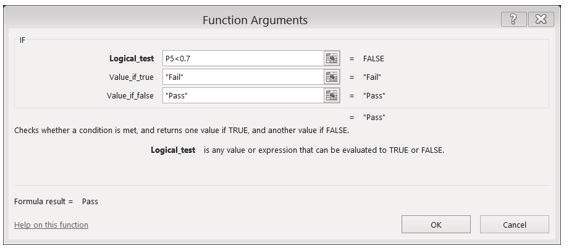
\includegraphics[width=\maxwidth{.95\linewidth}]{gfx/ch03_fig10}
	\caption{IF Function Dialog Box}
	\label{03:fig10}
\end{figure}

Notice that as each box is filled, Excel offers a brief explanation of the contents (below the boxes.) In the lower left corner is the results of the calculation so it can be checked before the function is inserted in the cell. In this case, DeShae is passing the class. Below that is a link to Help on this function. Selecting this link will open Excel help for this function, along with detailed information on how it works.

\begin{enumbox}
	\begin{enumerate}
		\item Once the required arguments are entered and checked, press \fmtButton{OK}. 
		\item The text \textit{Pass} should be displayed in \fmtLoc{Q5} because DeShae is passing the class.
		\item Click on \fmtLoc{Q5}. The formula bar should display the \fmtButton{IF} calculation: \fmtTyping{$ =IF(P5<0.7 $,''Fail'',''Pass'')} (see Figure \ref{03:fig11}).
		\item Use the \fmtButton{Auto Fill Handle} to copy \fmtLoc{Q5} to \fmtLoc{Q6:Q24}.
	\end{enumerate}
\end{enumbox}
	
\begin{figure}[H]
	\centering
	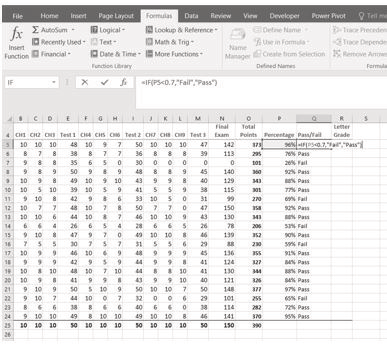
\includegraphics[width=\maxwidth{.95\linewidth}]{gfx/ch03_fig11}
	\caption{IF Function Results}
	\label{03:fig11}
\end{figure}

\subsection{Vlookup Function}

A \textit{VLOOKUP} function is used to look up information in a table. Sometimes that table is on a different sheet in the workbook, though it can be in another file entirely. In this case, all students' grades are determined by their percentage score. For this grade book, the table that relates a score to a grade is in $ A28 $:$ B32 $.

There are four pieces of information that are needed to build the \textit{VLOOKUP} function. 

\begin{itemize}
	\item The \textbf{Lookup\_value} is the value to look up. For this exercise, the lookup value will be the student's percentage score in \textit{Column P}.
	\item The \textbf{Table\_array} is the range (or table) where the lookup values are located. In this example the table of percentages and corresponding letter grades is in the range $ A28 $:$ B32 $. The lookup value, or percentage grade in this case, should always be in the first column in the table array for \textit{VLOOKUP} to work correctly. 
	\item The \textbf{Col\_index\_num} is the column number in the range that contains the value to return. In this example, $ A28 $:$ B32 $ is the \textit{Table\_array} range so \textit{Column A} is the first column (1), \textit{Column B} is the second column (2). To return the grade in \textit{Column B}, the number $ 2 $ would be entered as the \textit{Col\_index\_num}.
	\item The \textbf{Range\_lookup} is TRUE for an \textit{approximate} match or FALSE for an exact match. If this is left blank the default value is TRUE, or an approximate match.
\end{itemize}

Follow these steps to create the \textit{VLOOKUP} to display the correct \textit{Letter Grade} in \textit{Column R}.

\begin{enumbox}
	\begin{enumerate}
		\item Click in \fmtLoc{R5}.
		\item Click \fmtButton{Formulas $ \Rightarrow $ Function Library $ \Rightarrow $ Lookup \& Reference $ \Rightarrow $ VLOOKUP}. (See Figure \ref{03:fig12}).

		\begin{figure}[H]
			\centering
			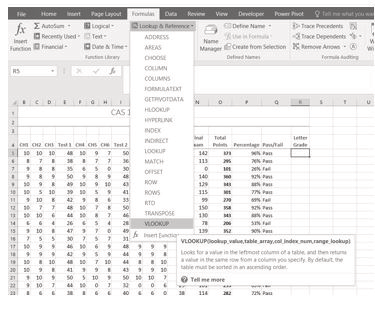
\includegraphics[width=\maxwidth{.95\linewidth}]{gfx/ch03_fig12}
			\caption{VLOOKUP Function}
			\label{03:fig12}
		\end{figure}
		
		\item Fill in the dialog box so that it looks like Figure \ref{03:fig13}.
		
		\begin{itemize}
			\item \textbf{Lookup\_value}. Specify the percentage score, which is in cell \fmtLoc{P5} for the first student.
			\item \textbf{Table\_array}. This is the range that contains the value to be returned by the function. In this case, that range is $ A28 $:$ B32 $. Note that this range does \textit{NOT} include the label in \textit{Row} $ 27 $, just the actual data. It is important that the cell references for the Table\_array need to be absolute: \fmtLoc{\$A\$28:\$B\$32}. When this function is copied to other cells the cell references should not change.
			\item \textbf{Col\_index\_number}. This is the column in the table array range that includes the information that should be returned. In this case, the grades are in the 2nd column of the range so the column index will be $ 2 $.
			\item \textbf{Range\_lookup}. Since an approximate match is appropriate for this application the default value of TRUE is appropriate. Since that is the default, nothing needs to be entered for this value. 
		\end{itemize}

		\item Be sure to observe the helpful definitions that Excel offers while filling in the \fmtButton{VLOOKUP} dialog box.
		\item When the dialog box is complete, press \fmtButton{OK}.
		\item The calculation in the formula bar is: \fmtTyping{=VLOOKUP(P5,\$A\$28:\$B\$32,2)}
		\item Use the \fmtButton{Auto Fill Handle} to copy \fmtLoc{R5} to \fmtLoc{R6:R24}.
	\end{enumerate}
\end{enumbox}
	
\begin{figure}[H]
	\centering
	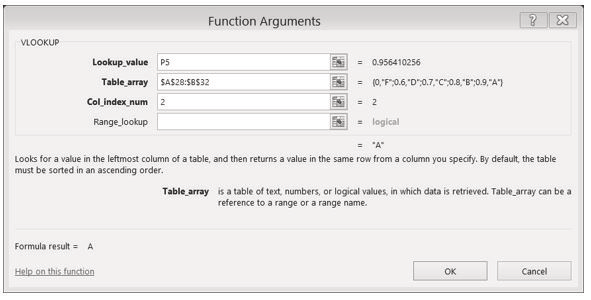
\includegraphics[width=\maxwidth{.95\linewidth}]{gfx/ch03_fig13}
	\caption{VLOOKUP completed dialog box}
	\label{03:fig13}
\end{figure}

Figure \ref{03:fig14} illustrates the grade book when the \textit{VLOOUP} function is applied.

\begin{figure}[H]
	\centering
	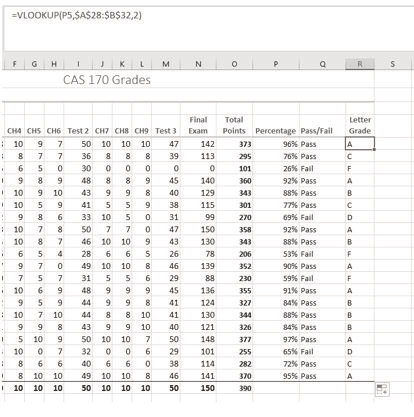
\includegraphics[width=\maxwidth{.95\linewidth}]{gfx/ch03_fig14}
	\caption{VLOOKUP Complete}
	\label{03:fig14}
\end{figure}

What if the \textit{VLOOKUP} function does not work as expected? In this case, a mistake was made in either the calculation of the \% scores in \textit{Column P} or there is an error in the \textit{VLOOKUP} function. To make repairs to the function, make sure that $ R5 $ is the active cell. On the Formula bar, press the \textit{Insert Function} button (see Figure \ref{03:fig15}). That will reopen the dialog box to make repairs. A common error is to forget to make the cell references for the \textit{Table\_array} absolute. Press \textit{OK} when the correction is completed and then recopy the corrected function.

\begin{figure}[H]
	\centering
	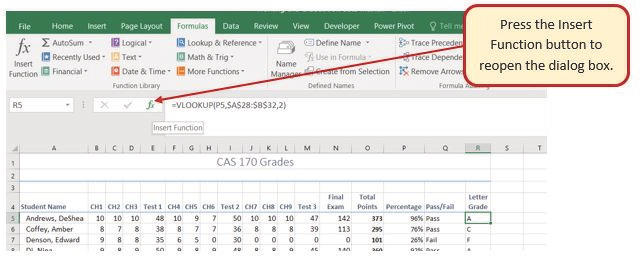
\includegraphics[width=\maxwidth{.95\linewidth}]{gfx/ch03_fig15}
	\caption{Insert Function}
	\label{03:fig15}
\end{figure}

\subsection{Error Messages}

Sometimes Excel notices errors in the calculations and may post a slightly mysterious error message. Table \ref{03:tab01} lists the common error messages that Excel displays along with their meanings\footnote{Table \ref{03:tab01} was adapted from  \url{https://www.dummies.com/software/microsoft-office/excel/understanding-excel-2010s-formula-error-values/}}.

\begin{table}[H]
	\rowcolors{1}{}{tablerow} % zebra striping background
	{\small
		%\fontsize{8}{10} \selectfont %Replace small for special font size
		\begin{longtable}{L{0.60in}L{3.65in}} %Left-aligned, Max width: 4.25in
			\textbf{Message} & \textbf{What Went Wrong} \endhead
			\hline
			\#DIV/$ 0 $ & The division operation refers to a cell that contains the value $ 0 $ or is blank.\\
			\#N/A & Technically, this is not an error value but a special value 		that can be manually entered into a cell to indicate that there is no value yet. This is a placeholder used while a spreadsheet is being developed.\\
			\#NAME? & This error value appears when a range name is incorrectly entered, or the name is deleted. Also, this commonly means that the formula is missing quotation marks around a text string.\\
			\#NULL & This error occurs if a space is used instead of a comma between ranges in function arguments. The formula needs to be carefully checked and corrected.\\
			\#NUM & This error is caused by an invalid argument in an Excel	function or by a formula that produces a number too large or too small for the worksheet.\\
			\#REF & This error occurs when a cell referred to in a formula has been deleted.\\
			\#VALUE & This error is most often the result of specifying a mathematical operation that refers to one or more cells that contain text.\\
			\rowcolor{captionwhite}
			\caption{Common Error Messages}
			\label{03:tab01}
		\end{longtable}
	} % End small
\end{table}

\subsection{Date Functions}

Very often dates and times are an important part of Excel data. Numbers that are correct today may not be accurate tomorrow, so it is frequently useful to include dates and times on the spreadsheets. Dates and times fall into two general categories.

\begin{itemize}
	\item \textbf{Remain the same.} For instance, if a spreadsheet includes data for May $ 15 $th then that date should not change each time the spreadsheet is accessed.
	\item \textbf{Change to reflect the current date/time.} When it is important to have the current date or time on a spreadsheet then Excel should update the information regularly.
\end{itemize}

Look at the functions at \textit{Formulas $ \Rightarrow $ Function Library $ \Rightarrow $ Date \& Time} (see Figure \ref{03:fig16}).

\begin{figure}[H]
	\centering
	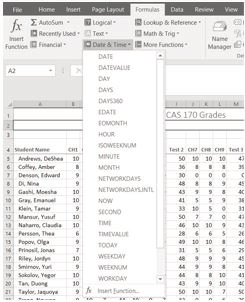
\includegraphics[width=\maxwidth{.95\linewidth}]{gfx/ch03_fig16}
	\caption{Date \& Time Functions}
	\label{03:fig16}
\end{figure}

For the grade book, the date and time should be displayed in $ A2 $, and it needs to be updated whenever the workbook file is opened.

\begin{enumbox}
	\begin{enumerate}
		\item Click in \fmtLoc{A2}. Notice that \fmtLoc{A2} extends all the way from \fmtLoc{Column A} to \fmtLoc{Column R}. Previously, the \fmtButton{Merge \& Center} tool was used on this cell to make it match the width of the title in \fmtLoc{Row 1}.
		\item Click \fmtButton{Formulas $ \Rightarrow $ Function Library $ \Rightarrow $ Date \& Time $ \Rightarrow $ NOW}. 
		\item Click \fmtButton{OK}.
		\item The result in the formula bar is: \fmtTyping{=NOW()} and the result in \fmtLoc{A2} depends on the current date and time. The \fmtButton{NOW} function is a very handy function; it takes no arguments and is volatile! That is not as alarming as it may seem. This just means that it does not need any information to do its job and the results will change frequently. 
		\item Wait at least one minute and then click in \fmtLoc{A2} and press \fmtKeystroke{F9} to update the time.
	\end{enumerate}
\end{enumbox}
	
Excel will update this field automatically whenever the file is saved, reopened, or printed. It may also happen more frequently than that, depending on how Excel is set up.

Another variation of the current date is the \textit{TODAY} function.

\begin{enumbox}
	\begin{enumerate}
		\item Click in \fmtLoc{A2}. Press \fmtKeystroke{Delete} to remove the \fmtButton{NOW} function.
		\item Click \fmtButton{Formulas $ \Rightarrow $ Function Library $ \Rightarrow $ Date \& Time $ \Rightarrow $ TODAY}. 
		\item Click \fmtButton{OK}.
		\item The result in the formula bar is \fmtTyping{=TODAY()} and the result in \fmtLoc{A2} is the current date. Since the time was not requested it is likely $ 12\!:\!00 $\textit{ AM}. That is not helpful, so the date format needs to be adjusted.
		\item Click \fmtButton{Home $ \Rightarrow $ Number $ \Rightarrow $ Number Format Launcher} (see Figure \ref{03:fig17}).
		\item In the \textit{Format Cells} dialog box, click the \textit{Number} tab. Choose the \fmtButton{Date} category and select the second option, \fmtButton{Wednesday, March 14, 2012} (this format is called \textit{Long Date}).
		\item Click \fmtButton{OK}.
		\item The current day and date should now be displayed in \fmtLoc{A2}.
	\end{enumerate}
\end{enumbox}
	
\begin{figure}[H]
	\centering
	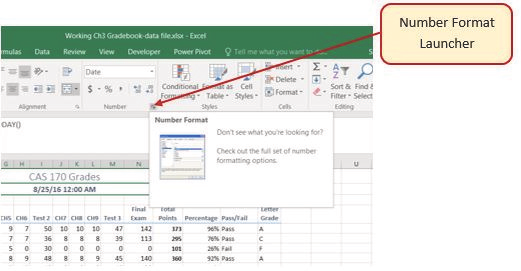
\includegraphics[width=\maxwidth{.95\linewidth}]{gfx/ch03_fig17}
	\caption{Number Format Launcher}
	\label{03:fig17}
\end{figure}

\begin{center}
	\begin{shtcutbox}{Keyboard Shortcuts}
		\textbf{Static Date and Time}
		\\
		\begin{itemize}
			\setlength{\itemsep}{0pt}
			\setlength{\parskip}{0pt}
			\setlength{\parsep}{0pt}

			\item \fmtKeystroke{CTRL} + \fmtKeystroke{;} (semicolon) inserts the current date
			\item \fmtKeystroke{CTRL} + \fmtKeystroke{:} (colon) inserts the current time.
			
		\end{itemize}
	\end{shtcutbox}
\end{center}


\begin{center}
	\begin{tkwbox}{Key Take-Aways}
		\textbf{Date Functions}
		\\
		\begin{itemize}
			\setlength{\itemsep}{0pt}
			\setlength{\parskip}{0pt}
			\setlength{\parsep}{0pt}

			\item Functions do not always have to be about arithmetic. Excel provides functions that helps perform logical evaluations, look things up, and work with dates and times.
			\item Excel displays error messages when formulas and functions are not constructed properly.
			
		\end{itemize}
	\end{tkwbox}
\end{center}

\section{Conditional Formatting}

\begin{center}
	\begin{objbox}{Learning Objectives}
		\begin{itemize}
			\setlength{\itemsep}{0pt}
			\setlength{\parskip}{0pt}
			\setlength{\parsep}{0pt}

			\item Use Conditional Formatting techniques to provide flexible highlighting or applying specified formatting only when certain conditions are met. Techniques include:

			\begin{itemize}			
				\item \textbf{Data bars}. Makes it easy to visualize values in a range of cells.
				\item \textbf{Cell Rules}. Highlights values that match specified requirements.
			\end{itemize}

		\end{itemize}
	\end{objbox}
\end{center}

\subsection{Initiating Conditional Formatting}

All necessary calculations are now in the \textit{CAS 170 Grades} spreadsheet. However, the grade book contains a lot of data. To make it easier to quickly find the most important pieces of data, Excel provides \textit{Conditional Formatting}.

\begin{enumbox}
	\begin{enumerate}
		\item Select the range \fmtLoc{O5:O24}.
		\item At the bottom of the selection, click on the \fmtButton{Quick Analysis Tool}. This is a popup tool with an icon that looks like a spreadsheet with colored lines.
		\item Click \fmtButton{Formatting $ \Rightarrow $ Data Bars} (see Figure \ref{03:fig18}).
	\end{enumerate}
\end{enumbox}
	
Excel places blue bars on top of the values; long blue bars for larger numbers, shorter ones for smaller numbers. This makes it easier to see how well each student did in the class immediately without having to look at the specific numbers.

\begin{figure}[H]
	\centering
	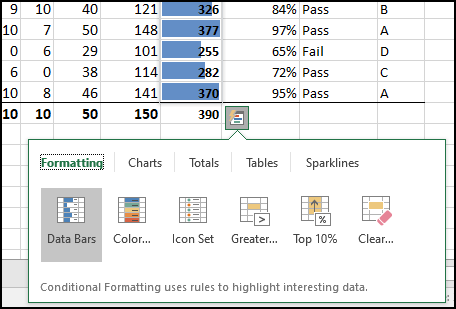
\includegraphics[width=\maxwidth{.95\linewidth}]{gfx/ch03_fig18}
	\caption{Data Bars on the Quick Analysis tool}
	\label{03:fig18}
\end{figure}

Following is another way to apply Data Bars.

\begin{enumbox}
	\begin{enumerate}
		\item Select the range \fmtLoc{O5:O24}.
		\item Click \fmtButton{Home $ \Rightarrow $ Styles $ \Rightarrow $ Conditional Formatting $ \Rightarrow $ Data Bars}. 	
		\item From there, data bars of different colors and opacities can be selected (see Figure \ref{03:fig19}).
	\end{enumerate}
\end{enumbox}
	
\begin{figure}[H]
	\centering
	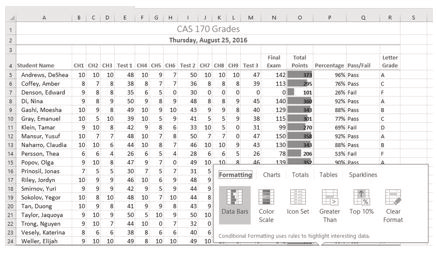
\includegraphics[width=\maxwidth{.95\linewidth}]{gfx/ch03_fig19}
	\caption{Data Bars on the Conditional Formatting tool}
	\label{03:fig19}
\end{figure}

It is even more important to highlight the students who are failing in the class, so that will be done in two places, the \textit{Percentages} and \textit{Letter Grade} columns. To start, any \textit{F} letter grades should be formatted with a light red fill color and dark red text.

\begin{enumbox}
	\begin{enumerate}
		\item Select the range \fmtLoc{R5:R24}.
		\item Click \fmtButton{Home $ \Rightarrow $ Styles $ \Rightarrow $ Conditional Formatting $ \Rightarrow $ Highlight Cells Rules} (see Figure \ref{03:fig20}).
		\item Select \fmtButton{Equal To}
		\item Enter \fmtTyping{F} in the \textit{Format cells that are EQUAL TO} text box, so those cells are highlighted with \fmtButton{Light Red Fill with Dark Red Text} (see Figure \ref{03:fig21}).
		\item Click \fmtButton{OK}.
	\end{enumerate}
\end{enumbox}
	
\begin{figure}[H]
	\centering
	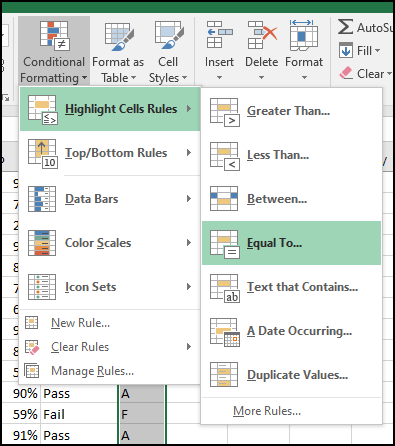
\includegraphics[width=\maxwidth{.95\linewidth}]{gfx/ch03_fig20}
	\caption{Conditional Formatting Equal To}
	\label{03:fig20}
\end{figure}

\begin{figure}[H]
	\centering
	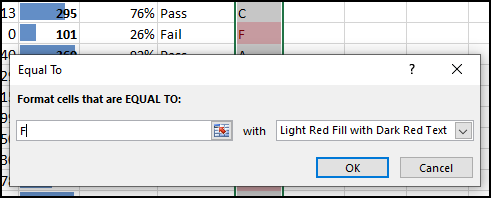
\includegraphics[width=\maxwidth{.95\linewidth}]{gfx/ch03_fig21}
	\caption{Conditional Formatting Equal To Dialog Box}
	\label{03:fig21}
\end{figure}

Now, highlight students who are passing the class. This time use the Pass/Fail text in the Pass/Fail column. If the text for a student is \textit{Pass} the cell should be formatted with a yellow fill and dark yellow text.

\begin{enumbox}
	\begin{enumerate}
		\item Select the range \fmtLoc{Q5:Q24}.
		\item Click \fmtButton{Home $ \Rightarrow $ Styles $ \Rightarrow $ Conditional Formatting $ \Rightarrow $ Highlight Cells Rules} (see Figure \ref{03:fig20}).
		\item Select \fmtButton{Equal To}
		\item Enter \fmtTyping{Pass} in the \textit{Format cells that are EQUAL TO} text box, so those cells are highlighted with \fmtButton{Yellow Fill with Dark Yellow Text}.
		\item Click \fmtButton{OK}.
	\end{enumerate}
\end{enumbox}
	
The default styles are a simple way to make specified data stand out, but any cell formatting can be set. When using custom cell formatting, it is probably a good idea to include other styling in addition to color. Remember that spreadsheets are often printed in black and white so conditional formatting that relies only on color would be lost. Next, use conditional formatting to display any \textit{Percentages} that are less than $ 60\% $ with red text formatted in bold and italic.

\begin{enumbox}
	\begin{enumerate}
		\item Select the range \fmtLoc{P5:P24}.
		\item Click \fmtButton{Home $ \Rightarrow $ Styles $ \Rightarrow $ Conditional Formatting $ \Rightarrow $ Highlight Cells Rules} (see Figure \ref{03:fig20}).
		\item Select \fmtButton{Less Than}
		\item Fill out the \textit{Less Than} dialog box so that cells that are less than $ 0.6 $ (that is 60\%) will have conditional formatting. Instead of using the default red text on a light red fill, press the down arrow at the end of the \textit{with} box and select \fmtButton{Custom Format}.
		\item On the \textit{Font} tab of the \textit{Format Cells} dialog box, in the \textit{Font style} box, select \fmtButton{Bold Italic}. In the \textit{Color} box, select \fmtButton{Red} (see Figure \ref{03:fig22}).
		\item Press \fmtButton{OK}. Then press \fmtButton{OK} again.
	\end{enumerate}
\end{enumbox}
	
\begin{figure}[H]
	\centering
	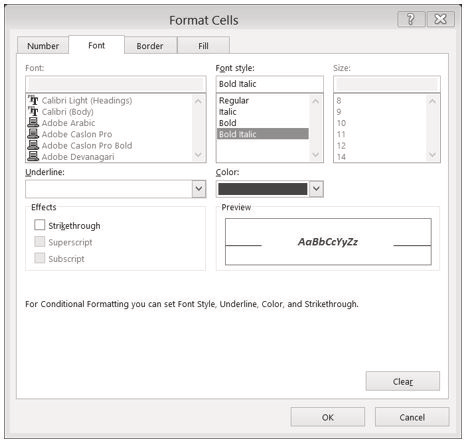
\includegraphics[width=\maxwidth{.95\linewidth}]{gfx/ch03_fig22}
	\caption{Conditional Formatting Custom Format Cells Dialog box}
	\label{03:fig22}
\end{figure}

Conditional Formatting is valuable since it reflects the current data and it changes whenever the data changes. To test this, delete DeShea's final exam score. (Click $ N5 $ then press \fmtKeystroke{Delete} on the keyboard.) Suddenly, DeShae is failing the course and the Conditional Formatting reflects that. Press \fmtKeystroke{CTRL} + \fmtKeystroke{Z} (Undo). The test score reappears, and the Conditional formatting reflects that as well.

\subsection{Modifying Conditional Formatting}

What if there is a mistake with the Conditional Formatting or it needs to be deleted altogether? Use the \textit{Conditional Formatting Manage Rules} tool. The following steps remove the conditional formatting rule that formats the \textit{Pass} text with yellow and modify the minimum passing percentage.

\begin{enumbox}
	\begin{enumerate}
		\item Click \fmtButton{Home $ \Rightarrow $ Styles $ \Rightarrow $ Conditional Formatting $ \Rightarrow $ Manage Rules}. 
		\item Select \fmtButton{This Worksheet} for \textit{Show formatting rules for} (see Figure \ref{03:fig23}).
		\item Since there is no need to highlight the students who are passing the class, click the second rule in the \textit{Rules Manager} (``Cell Value = 'Pass''') and press the \fmtButton{Delete Rule} button.
	\end{enumerate}
\end{enumbox}
	
\begin{figure}[H]
	\centering
	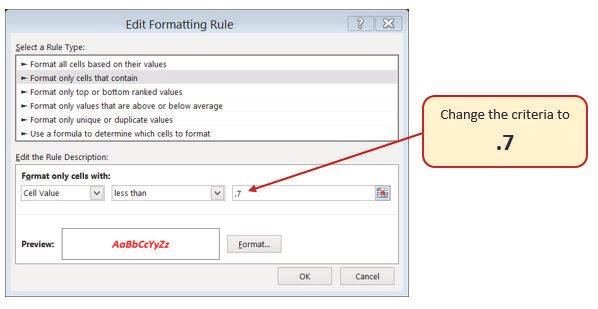
\includegraphics[width=\maxwidth{.95\linewidth}]{gfx/ch03_fig23}
	\caption{Conditional Formatting Manage Rules}
	\label{03:fig23}
\end{figure}

In a previous exercise (the \textit{IF} function), it was decided that students were failing if they got a percentage score of less than $ 70\% $, so the \textit{Conditional Formatting} rule in the \textit{Percentage} column needs to be changed to match that value.

\begin{enumbox}
	\begin{enumerate}
		\item Click the first rule, it reads \textit{Cell Value $ <0.6 $}.
		\item Click the \fmtButton{Edit Rule} button and change the $ 0.6 $ to $ 0.7 $ (see Figure \ref{03:fig24}).
		\item Click \fmtButton{OK} (or \fmtButton{Apply}) two times.
	\end{enumerate}
\end{enumbox}
	
\begin{figure}[H]
	\centering
	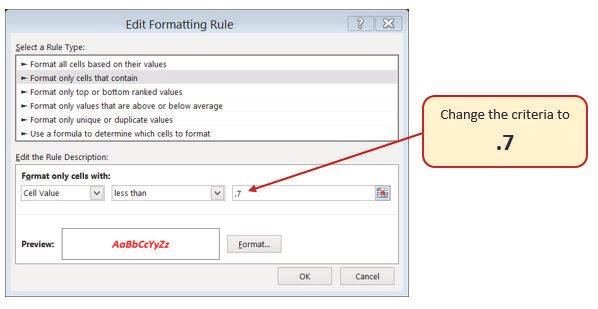
\includegraphics[width=\maxwidth{.95\linewidth}]{gfx/ch03_fig24}
	\caption{Conditional Formatting Edit Formatting Rule Dialog box}
	\label{03:fig24}
\end{figure}

Double check that the completed workbook matches Figure \ref{03:fig25}.

\begin{figure}[H]
	\centering
	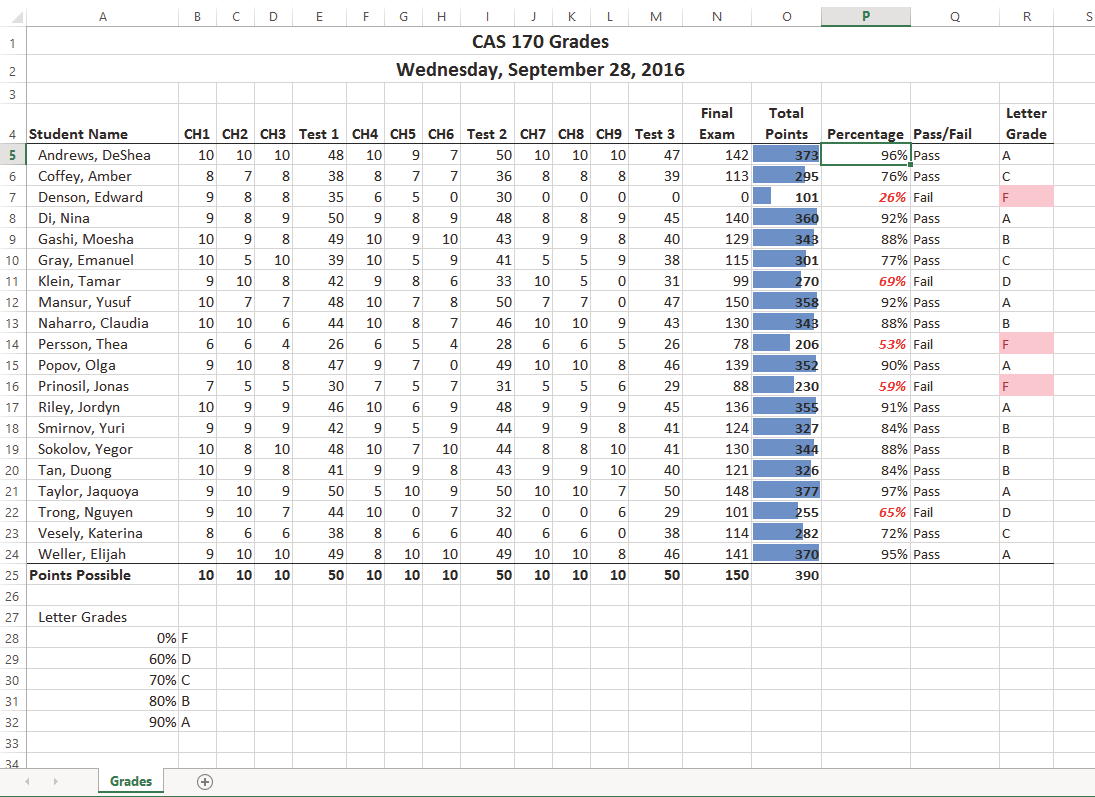
\includegraphics[width=\maxwidth{.95\linewidth}]{gfx/ch03_fig25}
	\caption{Completed Ch3-grade book}
	\label{03:fig25}
\end{figure}

\subsection{Setting the Print Area}

Before this workbook is finished, it needs to be prepared for printing. The first thing to do is set the \textit{Print Area} so that the table of \textit{Letter Grades} in $ A27 $:$ B32 $ does not print.

\begin{enumbox}
	\begin{enumerate}
		\item Select \fmtLoc{A1:R25}. This is the only part of the worksheet to be printed.
		\item Click \fmtButton{Page Layout $ \Rightarrow $ Page Setup $ \Rightarrow $ Print Area $ \Rightarrow $ Set Print Area}.
	\end{enumerate}
\end{enumbox}

Next, preview the worksheet in \textit{Print Preview} to check that the print area setting worked and to make sure it is printing on one page.

\begin{enumbox}
	\begin{enumerate}
		\item Click \fmtButton{File $ \Rightarrow $ Print}.
		\item Set the orientation to \fmtButton{Landscape}.
		\item Change the scaling so that the entire worksheet prints on one page.
		\item Close the print preview by clicking the arrow at the top left corner of the preview screen.
		\item Save the \fmtWorksheet{CH3-Grade Book} workbook.
		\item Compare the worksheet with the self-check answer key (\fmtWorksheet{CH3-Grade Book Solution}) and then close and submit the \fmtWorksheet{CH3-Grade Book} workbook as directed by the instructor.
	\end{enumerate}
\end{enumbox}
	
\section{Preparing to Print}

\begin{center}
	\begin{objbox}{Learning Objectives}
		\begin{itemize}
			\setlength{\itemsep}{0pt}
			\setlength{\parskip}{0pt}
			\setlength{\parsep}{0pt}

			\item Locate and fix formatting consistency errors.
			\item Apply new formatting techniques.
			\item Use Print Titles to repeat rows and columns on each page of a multiple page worksheet.
			\item Control where page breaks occur in a multiple page worksheet.
			
		\end{itemize}
	\end{objbox}
\end{center}

In this section, a worksheet will be reviewed for formatting consistency and two new formatting techniques are presented. The worksheet used in this section currently prints on four pages, so new page setup options are used to control how these pages print. 

\subsection{Reviewing Formatting for Consistency}

The workbook used for this exercise contains data about the national parks in the western United States. The workbook has been formatted but needs to be reviewed for consistency and prepared for printing. Figure \ref{03:fig26} shows how the second page of the finished worksheet will appear in \textit{Print Preview}.

\begin{figure}[H]
	\centering
	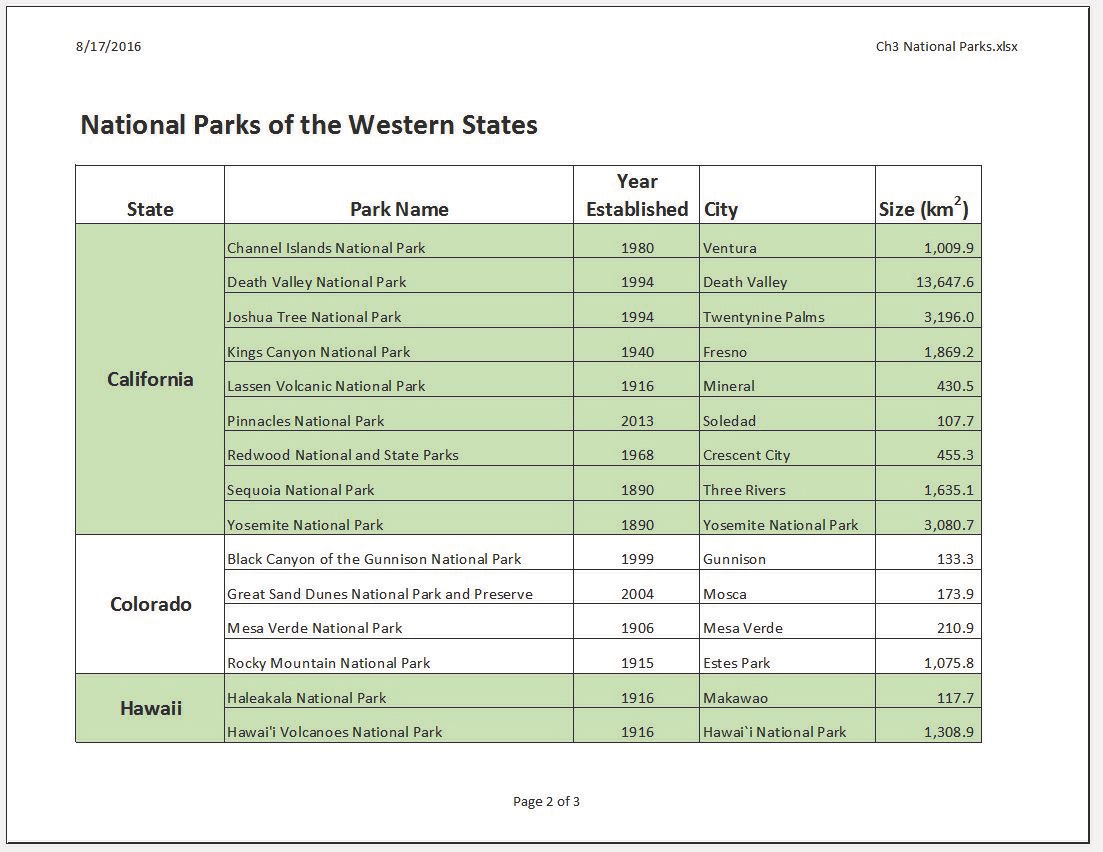
\includegraphics[width=\maxwidth{.95\linewidth}]{gfx/ch03_fig26}
	\caption{Completed National Parks worksheet}
	\label{03:fig26}
\end{figure}

\subsection{Reviewing Formatting for Inconsistencies}

The first thing to do is review the worksheet for formatting inconsistencies.

\begin{enumbox}
	\begin{enumerate}
		\item Open the data file named \fmtWorksheet{CH3-PTP Data} and use the \textit{File/Save As} command to save it as \fmtWorksheet{CH3-National Parks}.
		\item Scroll through the worksheet and locate the following formatting errors.
	
		\begin{itemize}
			\item The formatting of the \textit{Utah} label does not match the other states.
			\item The \textit{Year Established} values for \textit{Hawaii} are not center aligned like the other years.
			\item The cells for the \textit{Nevada} data should have the same green fill color as the other alternating states.
			\item The number of digits after the decimal place for the \textit{Size} values is inconsistent. Also, these values should be formatted with \textit{Comma} style to make them easier to read.
		\end{itemize}
	
		\item Complete the following steps to fix these errors.
	
		\begin{itemize}
			\item Select \fmtLoc{A34:A38}. 
			\item Click \fmtButton{Home $ \Rightarrow $ Alignment $ \Rightarrow $ Merge \& Center}.
			\item Change the font size to $ 16 $ and apply Bold format.
			\item Select \fmtLoc{C28:C29}.
			\item Click \fmtButton{Home $ \Rightarrow $ Alignment $ \Rightarrow $ Center}.
			\item Select \fmtLoc{A31:E31}.
			\item Apply a fill of \textit{Green, Accent $ 6 $, Lighter $ 60\% $}.
			\item Select \fmtLoc{E4:E43}. 
			\item Click \fmtButton{Home $ \Rightarrow $ Number $ \Rightarrow $ Comma}.
			\item Click \fmtButton{Home $ \Rightarrow $ Number $ \Rightarrow $ Decrease Decimal} until one digit appears after the decimal place for all values.
		\end{itemize}
		
		\item While these formatting errors are being corrected all typos should also be corrected.
	\end{enumerate}
\end{enumbox}
	
\subsection{Fine-Tuning Formatting}

Now that the formatting inconsistencies have been corrected, apply additional formatting techniques to make the worksheet look better. Start by vertically aligning the names of the states within the cells.

\begin{enumbox}
	\begin{enumerate}
		\item Select \fmtLoc{A4:A43} (the cells with the state labels).
		\item Click \fmtButton{Home $ \Rightarrow $ Alignment $ \Rightarrow $ Middle Align} (see Figure \ref{03:fig27}). Notice that the names of the states are now centered between the top and bottom borders of the cells.
	\end{enumerate}
\end{enumbox}
	
\begin{figure}[H]
	\centering
	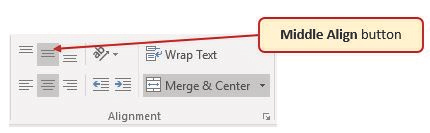
\includegraphics[width=\maxwidth{.95\linewidth}]{gfx/ch03_fig27}
	\caption{Alignment Group}
	\label{03:fig27}
\end{figure}

The next formatting correction is to change the label in $ E3 $ from \textit{Size (km2)} to \textit{Size (km\textsuperscript{2})} with the $ 2 $ after \textit{km} formatted as a superscript.

\begin{enumbox}
	\begin{enumerate}
		\item Double-click on cell \fmtLoc{E3} to enter \textit{Edit} mode
		\item Select just the $ 2 $ (be careful not to select anything else).
		\item Click \fmtButton{Home $ \Rightarrow $ Font $ \Rightarrow $ Dialog Box Launcher}. 	
		\item In the Effects section of the \textit{Format Cells} dialog box, check the box for \fmtButton{Superscript} (see Figure \ref{03:fig28}). 
		\item Click \fmtButton{OK}.
		\item Save the \fmtWorksheet{CH3-National Parks} file.
	\end{enumerate}
\end{enumbox}

\begin{figure}[H]
	\centering
	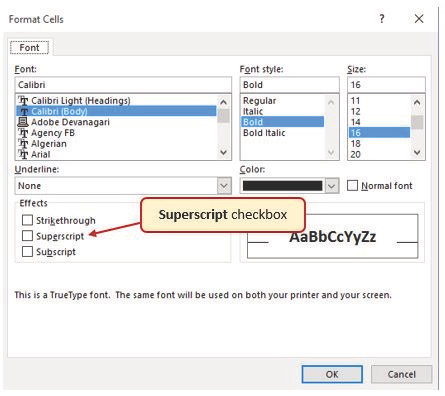
\includegraphics[width=\maxwidth{.95\linewidth}]{gfx/ch03_fig28}
	\caption{Font Tab in Format Cells Dialog Box}
	\label{03:fig28}
\end{figure}

\subsection{Repeating Column (And Row) Labels}

Now that the cell and text formatting are corrected, review the worksheet in \textit{Print Preview}. Notice that the worksheet is printing on multiple pages and it is not possible to know what each column of data represents on some of the pages.

\begin{enumbox}
	\begin{enumerate}
		\item With the \fmtWorksheet{CH3-National Parks} file still open, click \fmtButton{File $ \Rightarrow $ Print}.
		\item Click through each of the pages using the page number identifier at the bottom of the preview. The worksheet is currently printing on four pages, with the \textit{City} and \textit{Sizes} columns printing on separate pages from the rest of the data.
		\item Using the \fmtButton{Orientation} button on the left side of the preview, change the orientation to \textit{Landscape} to fit all the columns on one page. Unfortunately, the second and third pages have no column labels to identify the information in each column. 
		\item Exit \textit{Print Preview} by clicking the arrow button at the top left corner of the preview.
		\item Click \fmtButton{Page Layout $ \Rightarrow $ Page Setup $ \Rightarrow $ Print Titles}. The dialog box shown in Figure \ref{03:fig29} should appear.
	
		\begin{figure}[H]
			\centering
			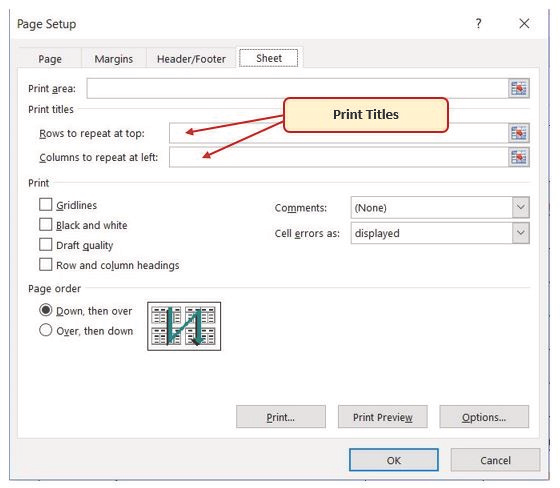
\includegraphics[width=\maxwidth{.95\linewidth}]{gfx/ch03_fig29}
			\caption{Print Titles}
			\label{03:fig29}
		\end{figure}

		\item Click the \fmtButton{Collapse Dialog} button next to the \textbf{Rows to repeat at top:} text box in the \textit{Page Setup} dialog box.
		\item In the worksheet, select \fmtLoc{Row $ 1 $}  through \fmtLoc{Row $ 3 $}.
		\item Press the \fmtKeystroke{Enter} key. This returns the \textit{Page Setup} dialog box to its expanded form. Notice that that the \textit{Rows to repeat at top} argument is now defined as $ \$1 $:$ \$3 $.
		\item Click \fmtButton{OK}.
	\end{enumerate}
\end{enumbox}

The worksheet does not change in Normal view, so return to \textit{Print Preview}. While in \textit{Print Preview}, notice that the pages are breaking in the middle of the information for a single park, but that will be corrected next.

\begin{enumbox}
	\begin{enumerate}
		\item Click \fmtButton{File $ \Rightarrow $ Print}. Notice that the first three rows are now repeated at the top of each page.
		\item Exit \textit{Print Preview} by clicking the arrow button at the top left corner of the preview.
	\end{enumerate}
\end{enumbox}

\begin{center}
	\begin{sklbox}{Skill Refresher}
		\textbf{Creating Print Titles}
		\\
		\begin{itemize}
			\setlength{\itemsep}{0pt}
			\setlength{\parskip}{0pt}
			\setlength{\parsep}{0pt}

			\item Open the \textit{Page Setup} dialog box and click the \textit{Sheet} tab.
			\item Click in the \textit{Rows to repeat at top:} box or the \textit{Columns to repeat at left:} box.
			\item Click in the worksheet and select the row(s) or column(s) to be repeated on each page.
						
		\end{itemize}
	\end{sklbox}
\end{center}

\subsection{Inserting Page Breaks}

Notice that the data for California is split between the first and second pages. Since it is desirable to keep all the data for each state on the same page, the page breaks need to be adjusted. Start by inserting a page break before the California data to force it to start on the second page, then move the page break for the third page if needed. To make these changes work in \textit{Page Break Preview}.

\begin{enumbox}
	\begin{enumerate}
		\item Click \fmtButton{View $ \Rightarrow $ Workbook Views $ \Rightarrow $ Page Break Preview}. The screen should be like Figure \ref{03:fig30}.
	\end{enumerate}
\end{enumbox}
	
\begin{figure}[H]
	\centering
	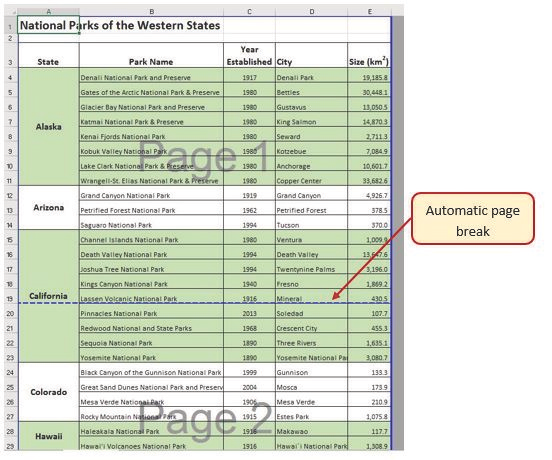
\includegraphics[width=\maxwidth{.95\linewidth}]{gfx/ch03_fig30}
	\caption{Page Break Preview}
	\label{03:fig30}
\end{figure}

In \textit{Page Break Preview}, automatic page breaks are displayed as dotted blue lines. Notice the dotted blue lines after \textit{Row} $ 20 $ and \textit{Row} $ 37 $, which indicate where Excel will start a new page. For this worksheet, the first page should break at the \textit{California} data, so insert a manual page break there.

\begin{enumbox}
	\begin{enumerate}
		\item Select cell \fmtLoc{A15}. When inserting a page break, select the cell \textit{below} where the page break should appear.
		\item Click \fmtButton{Page Layout $ \Rightarrow $ Page Setup $ \Rightarrow $ Breaks $ \Rightarrow $ Insert Page Break} (see Figure \ref{03:fig31}).
		\item There is now a solid blue line after \textit{Row} $ 14 $, which indicates a manual page break was inserted.
		\item Click \fmtButton{File $ \Rightarrow $ Print}. Notice that the California data now starts on the second page.
	\end{enumerate}
\end{enumbox}
	
\begin{figure}[H]
	\centering
	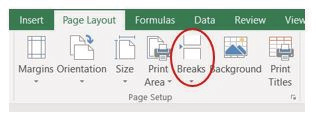
\includegraphics[width=\maxwidth{.95\linewidth}]{gfx/ch03_fig31}
	\caption{Breaks Button on Page Layout tab}
	\label{03:fig31}
\end{figure}

After looking at each page in \textit{Print Preview} it was decided that the third page should start with \textit{Montana}. To make this change, move the automatic page break that appears after \textit{Nevada}.

\begin{enumbox}
	\begin{enumerate}
		\item Exit \textit{Print Preview} by clicking the arrow button at the top left corner of the preview.
		\item Switch back to \textit{Page Break Preview} if needed.
		\item Locate the dotted blue line (automatic page break) after \fmtLoc{Row 31}.
		\item Put the pointer over the dotted blue line, and it will switch to a vertical double-headed arrow. Click on the dotted blue line and drag it above \fmtLoc{Row 30} (Montana).
		\item The line will now be a solid blue line, indicating a manual page break.
		\item Click \fmtButton{File $ \Rightarrow $ Print}. The Montana row now appears at the top of the third page.
	\end{enumerate}
\end{enumbox}
	
While evaluating the pages in \textit{Print Preview} it appears that there is too much white space at the bottom of the pages. To fix this, center the contents vertically on the pages.

\begin{enumbox}
	\begin{enumerate}
		\item Click the \fmtButton{Page Setup} link at the bottom of the \textit{Settings} section of \textit{Backstage View} to open the \textit{Page Setup} dialog box.
		\item Click on the \fmtButton{Margins} tab.
		\item In the \textit{Center on page} section, check the box for \fmtButton{Vertically} then click \fmtButton{OK}.
		\item Review each page in \textit{Print Preview} to see the changes. 
		\item Exit \textit{Print Preview} by clicking the arrow button at the top left corner of the preview.
	\end{enumerate}
\end{enumbox}
	
\subsection{Creating a Header and Footer Using Page Layout View}

Now that the worksheet is printing on three pages, with page breaks in appropriate places, it is time to add a header with the current date and filename. A footer will also be added with the page number and the total number of pages that will appear as \textit{Page 1 of 3}. 

\begin{enumbox}
	\begin{enumerate}
		\item Click \fmtButton{View $ \Rightarrow $ Workbook Views $ \Rightarrow $ Page Layout}. 
		\item The white space at the top of the worksheet should say \textit{Add header}. 
		\item Place the mouse pointer over the left section of the \textit{Header} and click to activate that section.
		\item Click \fmtButton{Header \& Footer Tools Design $ \Rightarrow $ Header \& Footer Elements $ \Rightarrow $ Current Date} (see Figure \ref{03:fig32}). Inserting the date this way will insert a field that will update every time the workbook is opened. (\fmtNewExcel{Excel 365} This tab is called \fmtButton{Header \& Footer}.)
		\item Place the mouse pointer over the right section of the \textit{Header} and click to activate that section.
		\item Click \fmtButton{Header \& Footer Tools Design $ \Rightarrow $ Header \& Footer Elements $ \Rightarrow $ Filename} (see Figure \ref{03:fig32}). Inserting the filename this way will insert a field that will update if the filename is changed.
		\item Click \fmtButton{Header \& Footer Tools Design $ \Rightarrow $ Navigation $ \Rightarrow $ Go to Footer}. 
		\item In the center section of the footer, type the word \fmtTyping{Page} with a space after it.
		\item Click \fmtButton{Header \& Footer Tools Design $ \Rightarrow $ Header \& Footer Elements $ \Rightarrow $ Page Number} (see Figure \ref{03:fig32}), then type a space after the \fmtTyping{\&[Page]} code that appears.
		\item Type the word \fmtTyping{of} with a space after it.
		\item Click \fmtButton{Header \& Footer Tools Design $ \Rightarrow $ Header \& Footer Elements $ \Rightarrow $ Number of Pages} (see Figure \ref{03:fig32}). The footer should match Figure \ref{03:fig33}.
		\item Click anywhere on the worksheet to close the \textit{Footer} editing.
		\item Click \fmtButton{File $ \Rightarrow $ Print}. Check that the date and file name are in the header and the page numbers in the footer are correct.
		\item Exit \textit{Print Preview} by clicking the arrow button at the top left corner of the preview.
		\item Save the \fmtWorksheet{CH3-National Parks} workbook.
		\item Compare the worksheet with the self-check answer key (\fmtWorksheet{CH3-National Parks Solution}) and then close and submit the \fmtWorksheet{CH3-National Parks} workbook as directed by the instructor.
	\end{enumerate}
\end{enumbox}
	
\begin{figure}[H]
	\centering
	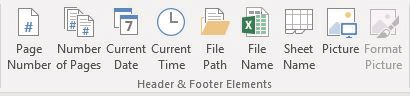
\includegraphics[width=\maxwidth{.95\linewidth}]{gfx/ch03_fig32}
	\caption{Header \& Footer Elements buttons}
	\label{03:fig32}
\end{figure}

\begin{figure}[H]
	\centering
	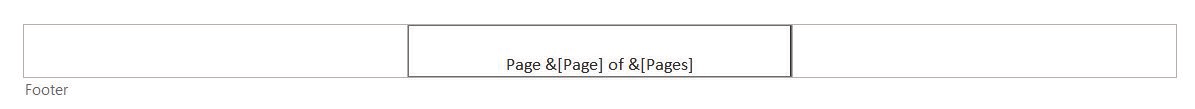
\includegraphics[width=\maxwidth{.95\linewidth}]{gfx/ch03_fig33}
	\caption{Completed Footer}
	\label{03:fig33}
\end{figure}

\begin{center}
	\begin{sklbox}{Skill Refresher}
		\textbf{Inserting Page Numbers}
		\\
		\begin{itemize}
			\setlength{\itemsep}{0pt}
			\setlength{\parskip}{0pt}
			\setlength{\parsep}{0pt}

			\item In Page Layout View, click in the section of the header or footer where the page number should appear.
			\item Type the word \textit{Page} followed by a space.
			\item Click \textit{Header \& Footer Tools Design $ \Rightarrow $ Header \& Footer Elements $ \Rightarrow $ Page Number}. This will create \textit{Page $ 1 $}.
			\item Type a space after the \textit{\&[Page]} code then type the word \fmtTyping{of} followed by a space. 
			\item Click \textit{Header \& Footer Tools Design $ \Rightarrow $ Header \& Footer Elements $ \Rightarrow $ Number of Pages}. This will create \textit{Page $ 1 $ of $ 4 $}.
			
		\end{itemize}
	\end{sklbox}
\end{center}

\begin{center}
	\begin{tkwbox}{Key Take-Aways}
		\textbf{Preparing to Print}
		\\
		\begin{itemize}
			\setlength{\itemsep}{0pt}
			\setlength{\parskip}{0pt}
			\setlength{\parsep}{0pt}

			\item Always check the formatting of worksheets for consistency.
			\item If a worksheet is printing on multiple pages, use \textit{Print Titles} to repeat rows at the top and/or columns at the left of every page to make it easier to interpret the data.
			\item Insert manual page breaks as needed in \textit{Page Break Preview} to control where a new page begins.
			\item Multiple page worksheets should include the page number in either the header or footer. Be sure to insert the Page Number element so that the correct page number will display on each page of the worksheet.
			
		\end{itemize}
	\end{tkwbox}
\end{center}

\section{Chapter Practice}

\subsection{Household Budget}

Elijah and Kelly Williams are a recently married couple living in Portland, Oregon. Elijah works part time and attends the local community college. Kelly works as a marketing manager at a clothing company in North Portland. They are trying to decide if they can afford to move to a better apartment, one that is closer to work and school. They want to use Excel to examine their household budget. They have started their budget spreadsheet, but they need help with it.

\begin{enumbox}
	\begin{enumerate}
	%fileopen PR3-Data
	%filesave PR3-Williams
		\item Open the file named \fmtWorksheet{PR3-Data} and then save it as \fmtWorksheet{PR3-Williams}.
		\item Insert two new rows at the top of the worksheet.
		\item Enter the following text in the indicated cells.
	
	\begin{itemize}
		\item \fmtLoc{A2}: \fmtTyping{Category}
		\item \fmtLoc{B2}: \fmtTyping{Item}
		\item \fmtLoc{C2}: \fmtTyping{January}
		\item \fmtLoc{O2}: \fmtTyping{Yearly Total} (adjust column width as needed to fit this text)
	\end{itemize}
	
		\item Starting in \fmtLoc{C2}, use the \fmtButton{Auto Fill Handle} to fill in the months \textit{February} through \textit{December} in cells \fmtLoc{D2:N2}. Adjust the widths of \fmtLoc{Column C} to \fmtLoc{Column N} to $ 10 $.
		\item Select \fmtLoc{A2:O2}.
		\item Click \fmtButton{Home $ \Rightarrow $ Font $ \Rightarrow $ Bold}.
		\item Click \fmtButton{Home $ \Rightarrow $ Alignment $ \Rightarrow $ Center}. 
		\item Click \fmtLoc{A1} and enter \fmtTyping{Williams Family Budget}. 
		\item Select \fmtLoc{A1:O1}.
		\item Click \fmtButton{Home $ \Rightarrow $ Alignment $ \Rightarrow $ Merge \& Center}.
		\item Select \fmtLoc{A1:O1}.
		\item Click \fmtButton{Home $ \Rightarrow $ Font $ \Rightarrow $ Bold}.
		\item Click \fmtButton{Home $ \Rightarrow $ Font $ \Rightarrow $ 22 point}. 
	
		\item Fill the cells for fixed expenses.
		\begin{enumerate}
			\item Copy \fmtLoc{C3:C4} and paste to \fmtLoc{D3:N4}.
			\item Copy \fmtLoc{C8:C9} and paste to \fmtLoc{D8:N9}.
			\item Copy \fmtLoc{C25} and paste to \fmtLoc{D25:N25}.
			\item Copy \fmtLoc{C27} and paste to \fmtLoc{D27:N27}.
			\item Copy \fmtLoc{C41} and paste to \fmtLoc{D41:N41}.
		\end{enumerate}	
		
		\item Select \fmtLoc{O3:O44}.
		\item Click \fmtButton{Formulas $ \Rightarrow $ Function Library $ \Rightarrow $ AutoSum}. 
		\item Delete the formulas from \fmtLoc{O7}, \fmtLoc{O17}, \fmtLoc{O24}, \fmtLoc{O32}, and \fmtLoc{O38}.
	
		% Calculated totals for each section
		\item Select \fmtLoc{C6}.
		\item Click \fmtButton{Formulas $ \Rightarrow $ Function Library $ \Rightarrow $ AutoSum}. Make certain that Excel selects \fmtLoc{C3:C5} for the \textit{AutoSum} function then press \fmtKeystroke{Enter}. This will calculate the \textit{Total Income} for January.
		\item Use the \fmtButton{Auto Fill Handle} to copy \fmtLoc{C6} to \fmtLoc{D6:O6}.
	
		\item Select \fmtLoc{C16}.
		\item Click \fmtButton{Formulas $ \Rightarrow $ Function Library $ \Rightarrow $ AutoSum}. Make certain that Excel selects \fmtLoc{C8:C15} for the \textit{AutoSum} function then press \fmtKeystroke{Enter}. This will calculate the \textit{Total Home Expenses} for January.
		\item Use the \fmtButton{Auto Fill Handle} to copy \fmtLoc{C16} to \fmtLoc{D16:O16}.
		
		\item Select \fmtLoc{C23}.
		\item Click \fmtButton{Formulas $ \Rightarrow $ Function Library $ \Rightarrow $ AutoSum}. Make certain that Excel selects \fmtLoc{C18:C22} for the \textit{AutoSum} function then press \fmtKeystroke{Enter}. This will calculate the \textit{Total Daily Living Expenses} for January.
		\item Use the \fmtButton{Auto Fill Handle} to copy \fmtLoc{C23} to \fmtLoc{D23:O23}.
		
		\item Select \fmtLoc{C31}.
		\item Click \fmtButton{Formulas $ \Rightarrow $ Function Library $ \Rightarrow $ AutoSum}. Make certain that Excel selects \fmtLoc{C25:C30} for the \textit{AutoSum} function then press \fmtKeystroke{Enter}. This will calculate the \textit{Total Transportation Expenses} for January.
		\item Use the \fmtButton{Auto Fill Handle} to copy \fmtLoc{C31} to \fmtLoc{D31:O31}.
	
		\item Select \fmtLoc{C37}.
		\item Click \fmtButton{Formulas $ \Rightarrow $ Function Library $ \Rightarrow $ AutoSum}. Make certain that Excel selects \fmtLoc{C33:C36} for the \textit{AutoSum} function then press \fmtKeystroke{Enter}. This will calculate the \textit{Total Entertainment Expenses} for January.
		\item Use the \fmtButton{Auto Fill Handle} to copy \fmtLoc{C37} to \fmtLoc{D37:O37}.
	
		\item Select \fmtLoc{C45}.
		\item Click \fmtButton{Formulas $ \Rightarrow $ Function Library $ \Rightarrow $ AutoSum}. Make certain that Excel selects \fmtLoc{C39:C44} for the \textit{AutoSum} function then press \fmtKeystroke{Enter}. This will calculate the \textit{Total Personal Expenses} for January.
		\item Use the \fmtButton{Auto Fill Handle} to copy \fmtLoc{C45} to \fmtLoc{D45:O45}.
		
		% Format for Total rows
		\item Select \fmtLoc{C3:O3}.
		\item Click \fmtButton{Home $ \Rightarrow $ Number $ \Rightarrow $ Accounting}.
		\item Click \fmtButton{Home $ \Rightarrow $ Number $ \Rightarrow $ Decrease Decimal} until there are no decimal places displayed.
		\item Click \fmtButton{Home $ \Rightarrow $ Font $ \Rightarrow $ Top Border} 
		
		\item Select \fmtLoc{C16:O16}.
		\item Click \fmtButton{Home $ \Rightarrow $ Number $ \Rightarrow $ Accounting}.
		\item Click \fmtButton{Home $ \Rightarrow $ Number $ \Rightarrow $ Decrease Decimal} until there are no decimal places displayed.
		\item Click \fmtButton{Home $ \Rightarrow $ Font $ \Rightarrow $ Top Border} 
	
		\item Select \fmtLoc{C23:O23}.
		\item Click \fmtButton{Home $ \Rightarrow $ Number $ \Rightarrow $ Accounting}.
		\item Click \fmtButton{Home $ \Rightarrow $ Number $ \Rightarrow $ Decrease Decimal} until there are no decimal places displayed.
		\item Click \fmtButton{Home $ \Rightarrow $ Font $ \Rightarrow $ Top Border} 
	
		\item Select \fmtLoc{C31:O31}.
		\item Click \fmtButton{Home $ \Rightarrow $ Number $ \Rightarrow $ Accounting}.
		\item Click \fmtButton{Home $ \Rightarrow $ Number $ \Rightarrow $ Decrease Decimal} until there are no decimal places displayed.
		\item Click \fmtButton{Home $ \Rightarrow $ Font $ \Rightarrow $ Top Border} 
	
		\item Select \fmtLoc{C37:O37}.
		\item Click \fmtButton{Home $ \Rightarrow $ Number $ \Rightarrow $ Accounting}.
		\item Click \fmtButton{Home $ \Rightarrow $ Number $ \Rightarrow $ Decrease Decimal} until there are no decimal places displayed.
		\item Click \fmtButton{Home $ \Rightarrow $ Font $ \Rightarrow $ Top Border} 
	
		\item Select \fmtLoc{C45:O45}.
		\item Click \fmtButton{Home $ \Rightarrow $ Number $ \Rightarrow $ Accounting}.
		\item Click \fmtButton{Home $ \Rightarrow $ Number $ \Rightarrow $ Decrease Decimal} until there are no decimal places displayed.
		\item Click \fmtButton{Home $ \Rightarrow $ Font $ \Rightarrow $ Top Border} 
	
		% The comma format for number cells
		\item Select \fmtLoc{C4:O5}.
		\item Click \fmtButton{Home $ \Rightarrow $ Number $ \Rightarrow $ Comma}.
		\item Click \fmtButton{Home $ \Rightarrow $ Number $ \Rightarrow $ Decrease Decimal} until there are no decimal places displayed.
	
		\item Select \fmtLoc{C8:O15}.
		\item Click \fmtButton{Home $ \Rightarrow $ Number $ \Rightarrow $ Comma}.
		\item Click \fmtButton{Home $ \Rightarrow $ Number $ \Rightarrow $ Decrease Decimal} until there are no decimal places displayed.
	
		\item Select \fmtLoc{C18:O22}.
		\item Click \fmtButton{Home $ \Rightarrow $ Number $ \Rightarrow $ Comma}.
		\item Click \fmtButton{Home $ \Rightarrow $ Number $ \Rightarrow $ Decrease Decimal} until there are no decimal places displayed.
	
		\item Select \fmtLoc{C25:O30}.
		\item Click \fmtButton{Home $ \Rightarrow $ Number $ \Rightarrow $ Comma}.
		\item Click \fmtButton{Home $ \Rightarrow $ Number $ \Rightarrow $ Decrease Decimal} until there are no decimal places displayed.
	
		\item Select \fmtLoc{C33:O36}.
		\item Click \fmtButton{Home $ \Rightarrow $ Number $ \Rightarrow $ Comma}.
		\item Click \fmtButton{Home $ \Rightarrow $ Number $ \Rightarrow $ Decrease Decimal} until there are no decimal places displayed.
	
		\item Select \fmtLoc{C39:O44}.
		\item Click \fmtButton{Home $ \Rightarrow $ Number $ \Rightarrow $ Comma}.
		\item Click \fmtButton{Home $ \Rightarrow $ Number $ \Rightarrow $ Decrease Decimal} until there are no decimal places displayed.
	
		\item Click \fmtLoc{A47} and enter \fmtTyping{Total Expenses}.
		\item Click \fmtLoc{C47} and enter \fmtTyping{=SUM(C16,C23,C31,C37,C45)}
		\item Copy \fmtLoc{C47} to \fmtLoc{D47:O47}.
	
		\item Click \fmtLoc{A49}. 
		\item Enter \fmtTyping{NET INCOME}. 
		\item Click \fmtButton{Home $ \Rightarrow $ Font $ \Rightarrow $ Bold}.
		\item Click \fmtButton{Home $ \Rightarrow $ Alignment $ \Rightarrow $ Indent}.
	
		\item Click \fmtLoc{C49}.
		\item Enter \fmtTyping{=C6-C47}.
		\item Copy \fmtLoc{C49} to \fmtLoc{D49:O49}.
	
		\item Select \fmtLoc{C47:O47}.
		\item Click \fmtButton{Home $ \Rightarrow $ Number $ \Rightarrow $ Accounting}.
		\item Click \fmtButton{Home $ \Rightarrow $ Number $ \Rightarrow $ Decrease Decimal} until there are no decimal places displayed.
		\item Click \fmtButton{Home $ \Rightarrow $ Font $ \Rightarrow $ Bold}.
		
		\item Select \fmtLoc{C49:O49}.
		\item Click \fmtButton{Home $ \Rightarrow $ Number $ \Rightarrow $ Accounting}.
		\item Click \fmtButton{Home $ \Rightarrow $ Number $ \Rightarrow $ Decrease Decimal} until there are no decimal places displayed.
		\item Click \fmtButton{Home $ \Rightarrow $ Font $ \Rightarrow $ Bold}.
		\item Click \fmtButton{Home $ \Rightarrow $ Font $ \Rightarrow $ Top and Bottom Border} 
	
		\item Select \fmtLoc{C49:N49}. 
		\item Click \fmtButton{Home $ \Rightarrow $ Styles $ \Rightarrow $ Conditional Formatting $ \Rightarrow $ Data Bars $ \Rightarrow $ Gradient Fill Blue}.
		
		\item Click \fmtLoc{B50}. 
		\item Enter \fmtTyping{New Apartment?}. 
		\item Click \fmtLoc{C50}.
		\item Enter an \fmtButton{IF} statement in that displays the word \textit{No} if the amount in \fmtLoc{C49} is less than or equal to zero and \textit{Maybe} if the amount is greater than zero. Hint: remember that the words ``No'' and ``Maybe'' must be enclosed in quotes. 
		\item Copy \fmtLoc{C50} to \fmtLoc{D50:N50}.
	
		\item Check to see if the \fmtButton{IF} statement worked correctly in \fmtLoc{Row 50}. If the cells say \textit{No} when the data bar in the cell above it is red and \textit{Maybe} when the data bar in the cell above it is blue, then the \fmtButton{IF} statement is correct.
	
		\item Review the worksheet in \textit{Print Preview}. Make any changes needed to make the worksheet print with landscape orientation on one page.
	%filesave PR3-Williams
		\item Save the \fmtWorksheet{PR3-Williams} workbook.
	%fileclose PR3-Williams
	%filesolution PR3-Williams Solution
		\item Compare the result with the self-check answer key (\fmtWorksheet{PR3-Williams Solution}) and then close and submit the \fmtWorksheet{PR3-Williams} workbook as directed by the instructor.
	\end{enumerate}
\end{enumbox}
	
\section{Scored Assessment}

\subsection{Astrocoffee Company}

Cynthia McHenry owns a coffee supply company named \textit{AstroCoffee}. She needs some help writing the formulas for the order form she uses to invoice customers. Formulas are needed for all of the calculations on the form. Some of the more complex parts are determining if the customer will get a discount (based on the customer status) as well as the shipping charge (orders over \$200 get free shipping). Use \fmtButton{IF} functions for both of those calculations.

\begin{enumbox}
	\begin{enumerate}
		\item Open the \fmtWorksheet{SC3-Data} workbook and save it as \fmtWorksheet{SC3-AstroCoffee}.
		\item Enter the following order information.
	
		\begin{itemize}
			\item Order \#: 45676
			\item Order Date: use a function that displays the current date
		\end{itemize}
	
		\item Enter the following Billing Information.
	
		\begin{tabular}{l}
			\hline
			Edwina Copeland\\
			4270 Heron Way Portland, OR 97225\\
			503-779-1873\\
			edwina.copeland@hmail.com\\
			\hline
		\end{tabular}
		
		\item For the \textit{Shipping Information}, create formulas using cell references to display the corresponding information from the \textit{Billing Information} section. For example, the \textit{Customer} cell will display the name of the customer found in \fmtLoc{C11}.
		\item In the range \fmtLoc{B19:E22}, enter the following item orders:
		
		{\small
			\begin{longtable}{p{0.4in}p{2.10in}p{0.25in}p{0.5in}} %Max width: 4.25in
				\textbf{Item \#} & \textbf{Description} & \textbf{Qty} & \textbf{Unit Price}\endhead
				\hline \\
				K56 & Dark Mocha K-Cups (12 pack) & 1 & 10.99\\
				G03 & Decaf Dark Roast – Ground (1 lb.) & 3 & 12.99\\
				B07 & Dark Roast – Whole Bean (1 lb.) & 2 & 13.99\\
				K52 & Chai Latte K-Cups (12 pack) & 3 & 12.99\\
				\caption{AstroCoffee Orders}
				\label{03:tab02}
			\end{longtable}
		}
		
		\item In cell \fmtLoc{F19}, enter an \fmtButton{IF} function that tests whether the order quantity in cell \fmtLoc{D19} is greater than $ 0 $ (zero). lf it is, return the value of the Qty (in \fmtLoc{D19}) multiplied by the Unit Price (in \fmtLoc{E19}), otherwise, return no text by entering ``''.
		\item Copy/fill the formula in \fmtLoc{F19} \fmtLoc{F20:F25}. \textit{Hint:} be sure to copy the formula to all of the \textit{Item Total} cells, even if they are blank so the worksheet is prepared for orders with more items in the future.
		\item In cell \fmtLoc{F26}, calculate the sum of all of the Item Total cells.
		\item In cell \fmtLoc{F27}, use an \fmtButton{IF} function to calculate the discount amount for this order based on the customer's status (which is found in \fmtLoc{F16}). If the customer's status is \textit{Preferred}, the discount amount will be the \textit{Order Subtotal} times the discount percentage found in cell \fmtLoc{B29}; otherwise the discount amount will be $ 0 $ (zero). \textit{Hint:} a formula is needed for the \textit{Value if True} argument.
		\item Calculate the Discounted Total for this order in cell \fmtLoc{F28}. \textit{Hint:} Use a simple subtraction formula.
		\item In cell \fmtLoc{F29}, use an \fmtButton{IF} function to display the correct Shipping Charge, based on the amount of the \textit{Discounted Total}. If the \textit{Discounted Total} is greater than or equal to the \textit{Free Shipping Minimum} found in cell \fmtLoc{B28}, the Shipping Charge is $ 0 $ (zero), otherwise, the Shipping Charge is $ 5\% $ of the Discounted Total. \textit{Hint:} a formula is needed for the Value if False to calculate what $ 5\% $ of the Discounted Total will be.
		\item Calculate the \textit{Invoice Total} in cell \fmtLoc{F31}. \textit{Hint:} This will be the total of the \textit{Discounted Total} and the \textit{Shipping Charge}.
		\item Review the worksheet in \textit{Print Preview}. Make any changes needed to make the worksheet print on one page.
		\item Save and close the \fmtWorksheet{SC3-AstroCoffee} workbook.
		\item Submit the \fmtWorksheet{SC3-AstroCoffee} workbook as directed by the instructor.
	\end{enumerate}
\end{enumbox}
